\section{Simulation Experiments and Results}
\label{sec:experiments}
The simulation code is supplied with the paper \cite{code_active_inference_2026} so that readers can reproduce the experiments, vary the conditions, and inspect the resulting localization behavior directly.

This section is organized as a progression toward a real-robot test environment. This is evaluated in two complementary ways. First, convergence scenarios use many randomized trials to test whether the belief can recover from different initial field positions and reach centimeter-level localization without landmark ambiguity. Next, tracking scenarios test whether the belief remains stable over time while the robot moves under noise, dropout, limited field of view, obstruction, and landmark ambiguity.
\footnote{Simulations were run on a modest 11th Gen Intel Core i5-1135G7 laptop (2.40 GHz, 4 cores). The simulation required approximately 82 µs/step, corresponding to 12,200 steps/s. This is an indicative hardware-dependent measurement, not a benchmark.}
\begin{figure}[t]
    \centering
    \begin{minipage}[t]{0.55\linewidth}
        \vspace{0pt}
        \centering
        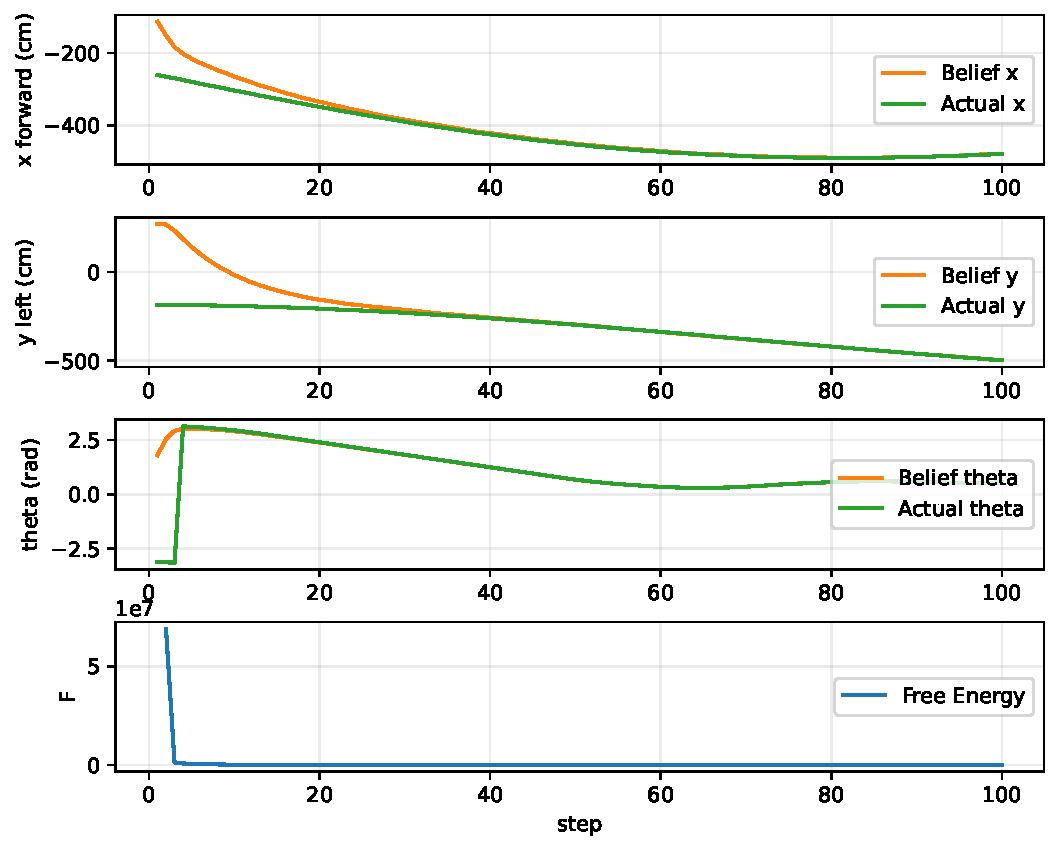
\includegraphics[width=0.95\linewidth,page=1]{figures/paper_experiment_20260909_172050.pdf}\\
        \small (a) Position tracking
    \end{minipage}
    \hfill
    \begin{minipage}[t]{0.42\linewidth}
        \vspace{0pt}
        \centering
        \includegraphics[width=0.95\linewidth,page=2]{figures/paper_experiment_20260909_172050.pdf}\\
        \small (b) Velocity traking

        \vspace{0.25em}

        \includegraphics[width=0.95\linewidth,page=3]{figures/paper_experiment_20260909_172050.pdf}\\
        \small (c) Acceleration tracking
    \end{minipage}
    \caption{\scriptsize Representative moving-robot belief estimate with noisy observations. Starting from random belief and actual poses, the belief converges to and tracks the actual pose in FCS as the robot follows a circular path. In (a), position and orientation are not observed directly; visible landmarks are observed in RCS $x$ and $y$, with bearing derived from these observations. In (b) and (c), velocity and acceleration observations in RCS are transformed to FCS using the belief heading. These plots illustrate that the update estimates generalized-coordinate dynamics rather than only pose.}
    \label{fig:typical-experiment-results}
\end{figure}
\FloatBarrier

\subsection{Static Robot Scenarios}
\label{subsec:experiments-static}

We first verify basic static convergence and progressively increase scenario complexity in subsequent sections. Here, the pose is inferred from unambiguous landmarks alone.
Table~\ref{tab:static-convergence-results} shows 100\% convergence from nearby and random initial positions, with varying numbers of visible landmarks and with or without dropout, noise, or both. In the near-start condition with 9 visible landmarks, convergence required only $23.6 \pm 5.0$ inference steps. Fewer available landmarks, noise or obstruction increased the number of inference steps needed for convergence.

\begin{table}[!htbp]
    \centering
    \caption{\scriptsize 100\% static robot convergence across a representative set covering nearby and random initial positions, varying visible landmark counts, and optional noise and dropout, using unique-ID data association. A trial is successful when the belief reaches the actual pose within 3 cm positional error and 3 degrees orientation error for at least five consecutive inference steps. Random: actual and initial belief poses sampled independently across the field, testing captured-robot-style recovery from an arbitrary wrong pose. Near: initial belief offset from the actual pose by at most 50 cm in x/y and 20 degrees in heading. Landmark-position noise in centimeters, landmark-angle noise in degrees.}
    \label{tab:static-convergence-results}
    \scriptsize
    \begin{tabular}{rrrrrlllll}
        \toprule
        N & Success & Mean & SD & P99 & Start & LM & Hz & Noise & Drop \\
        \midrule
        1000 & 100\% & 55.8 & 19.1 & 132 & Random & 9 & 40 & None & None \\
        1000 & 100\% & 23.6 & 5.0 & 36 & Near & 9 & 40 & None & None \\
        1000 & 100\% & 45.9 & 14.4 & 101 & Random & 9 & 200 & None & None \\
        1000 & 100\% & 63.9 & 22.1 & 149 & Random & 9 & 40 & 10 & 10\% \\
        1000 & 100\% & 129.4 & 85.3 & 467 & Random & 5 & 40 & None & None \\
        1000 & 100\% & 259.8 & 105.4 & 609 & Random & 2 & 40 & None & None \\
        1000 & 100\% & 48.2 & 20.4 & 113 & Near & 5 & 40 & 10 & 10\% \\
        1000 & 100\% & 112.0 & 40.7 & 225 & Near & 2 & 40 & 10 & 10\% \\
        \bottomrule
    \end{tabular}
\end{table}

\FloatBarrier

\subsection{Dynamic Robot Scenarios}
\label{subsec:experiments-dynamic}

The next question is whether the algorithm can converge while the actual robot is moving. Table~\ref{tab:dynamic-convergence-results} shows 100\% convergence across all tested dynamic scenarios. In the near-start condition with 9 visible landmarks, convergence required $44.2 \pm 22.4$ inference steps. The moving-robot results follow the same main trend as the static tests: fewer available landmarks, noise and obstruction increase the number of inference steps needed for convergence, but do not prevent recovery in these tests with unambiguous landmarks.
\footnote{For a kidnapped-robot-style recovery with only two unique landmarks visible at 40 Hz, 260 steps correspond to 6.5 s in the static case and 388 steps to 9.7 s in the dynamic case, which remains practical for recovery.}
The representative noisy run in Fig.~\ref{fig:typical-experiment-results} illustrates this behavior. The belief starts away from the actual pose, is corrected by motion and landmark prediction errors, and then remains close to the moving actual robot. The velocity and acceleration plots show that the update estimates a generalized-coordinate belief rather than only a static pose.

\begin{table}[!htbp]
    \centering
    \caption{\scriptsize 100\% dynamic-robot convergence. The robot follows random target trajectories, reaching speeds up to 5 m/s and accelerations up to 12 m/s$^2$. Tests use the same near/random starting position, landmark-visibility, noise, unique-ID data association, and dropout conditions as Table~\ref{tab:static-convergence-results}.}
    \label{tab:dynamic-convergence-results}
    \scriptsize
    \begin{tabular}{rrrrrlllll}
        \toprule
        N & Success & Mean & SD & P99 & Start & LM & Hz & Noise & Drop \\
        \midrule
        1000 & 100\% & 61.4 & 19.0 & 119 & Random & 9 & 40 & None & None \\
        1000 & 100\% & 44.2 & 22.4 & 105 & Near & 9 & 40 & None & None \\
        1000 & 100\% & 53.5 & 22.8 & 140 & Random & 9 & 200 & None & None \\
        1000 & 100\% & 74.9 & 28.2 & 163 & Random & 9 & 40 & 10 & 10\% \\
        1000 & 100\% & 121.2 & 57.4 & 308 & Random & 5 & 40 & None & None \\
        1000 & 100\% & 388.5 & 248.8 & 1313 & Random & 2 & 40 & None & None \\
        1000 & 100\% & 93.6 & 60.5 & 267 & Near & 5 & 40 & 10 & 10\% \\
        1000 & 100\% & 289.4 & 234.6 & 1157 & Near & 2 & 40 & 10 & 10\% \\
        \bottomrule
    \end{tabular}
\end{table}
\FloatBarrier

\subsection{Tracking Duration Test}
\label{subsec:experiments-visibility-stress}

Tracking duration tests shift the focus from convergence to sustained tracking under partial and interrupted landmark visibility. To approximate humanoid robot-soccer perception, landmark visibility is restricted to a representative 110-degree field of view, and the simulation includes 2-second obstruction periods in which other robots temporarily block relevant field landmarks.

Under the combined conditions of noise, dropout, limited field of view, and temporary obstruction, the method remained stable over a 2-hour Random targets run initialized from a near-start belief. The result is not error-free tracking at every instant, but stable recovery: motion terms keep the belief evolving during weak landmark evidence, and later landmark observations correct accumulated deviations. Table~\ref{tab:visibility-stress-tracking-summary} summarizes this behavior. The left panel reports the percentage of timesteps within each error threshold; the right panel shows that more visible landmarks correlate with lower mean absolute X error. Appendix~\ref{sec:appendix-landmark-tracking} provides a more detailed view of how landmark availability affects tracking error over time.

\begin{table}[!htbp]
    \centering
    \caption{\scriptsize Sustained tracking under challenging visibility conditions, demonstrated over two continuous hours at speeds up to5~m/s and accelerations up to 12~m/s$^2$, with observation noise, landmark dropout, a $110^\circ$ field of view, and temporary obstruction. The near-start Random targets run uses unique-ID landmark association at 40 Hz with 9 landmarks; while moving, the robot heading continuously rotates toward (300 cm, 0 cm). The run contains 288,000 inference timesteps (2 h at 40 Hz). Left: percentage of timesteps within each error threshold. For example, 39.44\% in the \(|x|\) column means that the absolute \(x\)-position error was at most 3 cm for 39.44\% of the timesteps. Right: Mean absolute X error, SD, and percentage of timesteps by visible landmark count during the two-hour tracking run. More visible landmarks correlate with lower error.}
    \label{tab:visibility-stress-tracking-summary}
    \scriptsize
    \begin{minipage}[t]{0.49\linewidth}
        \centering
        \textbf{(a) Tracking precision}\\[0.25em]
        \setlength{\tabcolsep}{5pt}
        \begin{tabular}{lccc}
            \toprule
            Band & $|x|$ & $|y|$ & $|\theta|$ \\
            \midrule
            3 cm / 1 deg & 39.44\% & 31.50\% & 94.25\% \\
            5 cm / 2 deg & 61.07\% & 50.26\% & 98.83\% \\
            7.5 cm / 3 deg & 79.64\% & 68.86\% & 99.69\% \\
            10 cm / 4 deg & 90.12\% & 81.73\% & 99.93\% \\
            15 cm / 5 deg & 97.86\% & 94.88\% & 99.99\% \\
            20 cm / 7.5 deg & 99.59\% & 98.73\% & 100.00\% \\
            25 cm / 10 deg & 99.90\% & 99.73\% & 100.00\% \\
            30 cm / 15 deg & 99.98\% & 99.96\% & 100.00\% \\
            \bottomrule
        \end{tabular}
    \end{minipage}
    \hfill
       \begin{minipage}[t]{0.49\linewidth}
        \centering
       \textbf{(b) X error by visible landmarks}\\[0.25em]
\setlength{\tabcolsep}{3pt}
\begin{tabular}{lccc}
    \toprule
    Visible LM & Mean $|x|$ (cm) & SD & Timestep \% \\
    \midrule
    0 & 6.38 & 5.13 & 0.12 \\
    1 & 5.83 & 4.76 & 1.77 \\
    2 & 5.55 & 4.55 & 8.11 \\
    3 & 5.28 & 4.20 & 16.88 \\
    4 & 4.92 & 3.93 & 27.32 \\
    5 & 4.58 & 3.66 & 25.56 \\
    6 & 4.13 & 3.19 & 15.09 \\
    7 & 4.00 & 3.20 & 3.34 \\
    8 & 3.83 & 2.94 & 1.44 \\
    9 & 3.46 & 2.67 & 0.35 \\
    \bottomrule
\end{tabular}
    \end{minipage}
\end{table}

\FloatBarrier

\subsection{Tracking Duration Test Under Landmark Ambiguity}
\label{subsec:experiments-landmark-ambiguity}

The next stress condition tests landmark ambiguity. Many soccer-field landmarks are geometrically repeated, so a local observation does not always identify a unique field location. For example, an observed field corner can correspond to any of the four physical field corners. This creates a data-association problem: the algorithm must decide which known FCS landmark generated the RCS observation before the prediction error can be used for belief updating.

In this proof of concept, ambiguity is handled with gated nearest-neighbor association. For each observed landmark type, candidate map landmarks of the same type are projected into RCS from the current belief; the closest candidate is selected only if its prediction error falls within a gating threshold. Otherwise, the observation is rejected for that update step. This is a deliberately simple and pragmatic association strategy. Although more advanced multi-hypothesis approaches were considered, the simulations showed that gated nearest-neighbor matching was sufficient for the present proof of concept. With landmark ambiguity enabled, the method maintained stable tracking when initialized from a converged belief.


\begin{table}[!htbp]
    \centering
    \caption{\scriptsize Sustained tracking under the challenging conditions of
Table~\ref{tab:visibility-stress-tracking-summary}, with landmark ambiguity.}
    \label{tab:landmark-ambiguity-tracking}
    \scriptsize
    \setlength{\tabcolsep}{5pt}
    \begin{tabular}{lccc}
        \toprule
        Band & $|x|$ & $|y|$ & $|\theta|$ \\
        \midrule
        3 cm / 1 deg & 39.05\% & 31.37\% & 94.00\% \\
        5 cm / 2 deg & 60.09\% & 50.21\% & 98.82\% \\
        7.5 cm / 3 deg & 78.71\% & 68.57\% & 99.71\% \\
        10 cm / 4 deg & 89.69\% & 81.74\% & 99.93\% \\
        15 cm / 5 deg & 97.67\% & 94.63\% & 99.98\% \\
        20 cm / 7.5 deg & 99.58\% & 98.47\% & 100.00\% \\
        25 cm / 10 deg & 99.97\% & 99.65\% & 100.00\% \\
        30 cm / 15 deg & 100.00\% & 99.93\% & 100.00\% \\
        \bottomrule
    \end{tabular}
\end{table}
\FloatBarrier
